% !TeX root=../main.tex

\chapter{پاسخ سوالات سری اول}

% دستور زیر باعث عدم‌نمایش شماره صفحه در اولین صفحهٔ این فصل می‌شود.
%\thispagestyle{empty}
\section{ پاسخ سوال 1}

\subsection{بخش 1}

\subsubsection{قسمت یک}
برای حل این مسئله ی بهینه سازی، با استفاده از یک کد متلب ابتدا نابرابری های داده شده در یک نمودار دو بعدی ترسیم شده و ناحیه ی اشتراک حاصل از این خطوط  برای پاسخ های ممکن به دست می آید.

\begin{latin}
	\begin{lstlisting}[frame=single,style=Matlab-Pyglike]
		
% Solve pairs of equations symbolically for intersections
syms x1 x2

% Line equations:
eq1 = x1 + 2*x2 == 8;          % From x1 + 2*x2 = 8
eq2 = 3*x1 + 2*x2 == 12;       % From 3*x1 + 2*x2 = 12
eq3 = x1 + x2 == 4;            % From x1 + x2 = 4

% Solve intersections
% Intersection of eq1 and eq2
sol_1_2 = solve([eq1, eq2], [x1, x2]);

% Intersection of eq1 and eq3
sol_1_3 = solve([eq1, eq3], [x1, x2]);

% Intersection of eq2 and eq3
sol_2_3 = solve([eq2, eq3], [x1, x2]);

% Step 2: Identify intercepts with axes
% x1 intercepts and x2 intercepts
intercept_x1 = solve(eq1, x1);   % x1-intercept of x1 + 2*x2 = 8
intercept_x2 = solve(eq2, x1);   % x1-intercept of 3*x1 + 2*x2 = 12

% Boundary points on axes
boundary_points = [0, 8/2; 4, 0]; % Intersections with axes: (0, 8/2), (4, 0)

% Collect all intersection points
points = [
double([sol_1_2.x1, sol_1_2.x2]);  % Intersection of eq1 and eq2
double([sol_1_3.x1, sol_1_3.x2]);  % Intersection of eq1 and eq3
double([sol_2_3.x1, sol_2_3.x2]);  % Intersection of eq2 and eq3
boundary_points                     % Intersection with axes
];

% Step 3: Objective function
f = @(x1, x2) 5*x1 + 6*x2;

% Evaluate the objective function at each point
f_vals = arrayfun(@(i) f(points(i, 1), points(i, 2)), 1:size(points, 1));

% Find the minimum value and corresponding point
[min_val, min_idx] = min(f_vals);
optimal_point = points(min_idx, :);

% Display the results
fprintf('Intersection points and corresponding function values:\n');
for i = 1:size(points, 1)
fprintf('Point (x1 = %.2f, x2 = %.2f), f(x1, x2) = %.2f\n', points(i, 1), points(i, 2), f_vals(i));
end
fprintf('Optimal point: (x1 = %.2f, x2 = %.2f), Minimum f(x1, x2) = %.2f\n', optimal_point(1), optimal_point(2), min_val);

% Step 4: Plot the feasible region and the intersection points
figure; hold on;

% Plot the feasible region
contourf(X1, X2, feasible_region, [1 1], 'FaceColor', 'r', 'EdgeColor', 'none');

% Plot the lines representing the inequalities
plot(x1_vals, (8 - x1_vals)/2, 'b', 'LineWidth', 1.5);     % x1 + 2*x2 = 8
plot(x1_vals, (12 - 3*x1_vals)/2, 'g', 'LineWidth', 1.5);  % 3*x1 + 2*x2 = 12
plot(x1_vals, 4 - x1_vals, 'm', 'LineWidth', 1.5);         % x1 + x2 = 4

% Plot intersection points
plot(points(:, 1), points(:, 2), 'ko', 'MarkerFaceColor', 'y', 'MarkerSize', 5);

% Highlight the optimal point
plot(optimal_point(1), optimal_point(2), 'ro', 'MarkerFaceColor', 'r', 'MarkerSize', 10);

% Add labels and title
xlabel('x1');
ylabel('x2');
title('Feasible Region and Intersection Points');
grid on;
hold off;

xlim([0 ])
ylim([0.0 10])
		
	\end{lstlisting}
\end{latin}

% TODO: \usepackage{graphicx} required
\begin{figure}
	\centering
	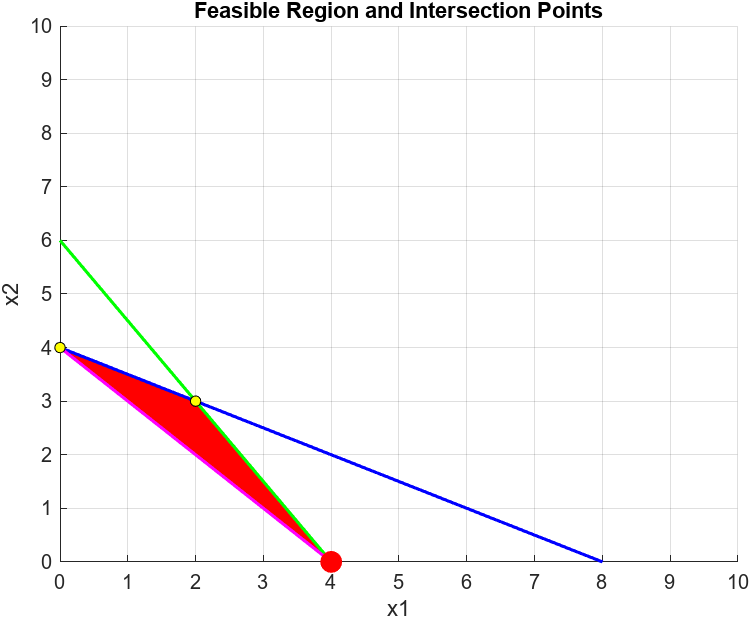
\includegraphics[width=1\linewidth]{../img/Q1_1}
	\caption{}
	\label{fig:q11}
\end{figure}

پاسخ بهینه برای معادله ی 
	\( f(x_1, x_2) = 5x_1 + 6x_2 \)
با جایگذاری مقادیر ممکن در معادله به دست می آید.
	
	\begin{itemize}
		\item \( (x_1 = 2.00, x_2 = 3.00) \), \( f(x_1, x_2) = 28.00 \)
		\item \( (x_1 = 0.00, x_2 = 4.00) \), \( f(x_1, x_2) = 24.00 \)
		\item \( (x_1 = 4.00, x_2 = 0.00) \), \( f(x_1, x_2) = 20.00 \)
		\item \( (x_1 = 0.00, x_2 = 4.00) \), \( f(x_1, x_2) = 24.00 \)
		\item \( (x_1 = 4.00, x_2 = 0.00) \), \( f(x_1, x_2) = 20.00 \)
	\end{itemize}
	
جواب بهینه برای این سوال برابر خواهد بود با:
	\[
	(x_1 = 4.00, x_2 = 0.00) , \quad f(x_1, x_2) = 20.00
	\]
\subsubsection{قسمت دو}
در این مرحله، با استفاده از ابزار های 
Yalmip
, 
CVX
مسئله ی بهینه سازی را حل می کنیم. در بخش اول، با استفاده از کد متلب زیر، محدودیت ها و تابع هزینه تعریف شده و در نهایت با اجرای کد، جواب های مورد نظر به دست می آید.

\begin{latin}
	\begin{lstlisting}[frame=single,style=Matlab-Pyglike]
		
yalmip('clear')
x1 = sdpvar(1,1)
x2 = sdpvar(1,1)

constraints = [x1<=8-2*x2 , 3*x1 + 2*x2<= 12, x1 + x2>=4 , x1>=0 , x2 >=0]

obj = 5*x1 + 6*x2

sol = optimize(constraints , obj)

if sol.problem ==0
val1 = value(x1)
val2 = value(x2)
objvalue = value(obj)
end
		
	\end{lstlisting}
\end{latin}

با استفاده از این کد، در نهایت جواب هایی مطابق با آنچه که به روش تحلیلی به دست آمد، حاصل می شود.

\[
(x_1 = 4.00, x_2 = 0.00) , \quad f(x_1, x_2) = 20.00
\]
در گام بعد، با استفاده از پکیج CVX، بار دیگر این مسئله حل می شود.


\begin{latin}
	\begin{lstlisting}[frame=single,style=Matlab-Pyglike]
		
cvx_begin

variables x1 x2

% Objective function
minimize(5*x1 + 6*x2)

% Subject to the constraints
subject to
x1 + 2*x2 <= 8
3*x1 + 2*x2 <= 12
x1 + x2 >= 4
x1 >= 0
x2 >= 0

cvx_end

% Display the results
x1_value = x1
x2_value = x2

		
	\end{lstlisting}
\end{latin}

\[
(x_1 = 4.00, x_2 = 0) , \quad f(x_1, x_2) = 20.00
\]

مشاهده می شود که با استفاده از این روش نیز، پاسخ مشابهی به دست می آید.

\subsection{بخش 2}
در این بخش، مشابه آنچه که در بخش پیشین انجام شد، ابتدا به روش تحلیلی و با رسم ناحیه ی نقاط امکان پذیری، نقاط بهینه تشخیص داده می شوند.
در کد متلب زیر، با تعیین معادلات مربوط به محدودیت ها، و محاسبه ی نقاط تقاطع خطوط، پاسخ بهینه به دست آمده و نمایش داده شده است.

\begin{latin}
	\begin{lstlisting}[frame=single,style=Matlab-Pyglike]
		
% Clear previous variables
clear; clc;

% Step 1: Define symbolic variables
syms x1 x2;

% Step 2: Define the constraints
% Lines based on constraints
eq1 = x1 + x2 == -20;  % From x1 + x2 = -20
eq2 = x1 + x2 == 5;    % From x1 + x2 = 5

% Step 3: Solve intersections
% Intersection of eq1 and eq2
sol_1_2 = solve([eq1, eq2], [x1, x2]);

% Define boundaries for x1 and x2
boundary_x1 = [-5, 5];  % x1 boundaries
boundary_x2 = [-1, 5];  % x2 boundaries

% Collect boundary points based on the constraints
boundary_points = [
-5, -1;   % Bottom left corner
-5, 5;    % Top left corner
5, -1;    % Bottom right corner
0, 5;     % Top right corner
5,0
];

% Collect all intersection points (if valid)
points = [
double([sol_1_2.x1, sol_1_2.x2]);  % Intersection of eq1 and eq2
boundary_points                     % Intersections with axes
];

% Step 4: Define the objective function
f = @(x1, x2) abs(x1 - 5) + abs(x2 - 5);

% Step 5: Evaluate the objective function at each point
% Filter valid points based on constraints
valid_points = points((points(:,1) >= boundary_x1(1)) & (points(:,1) <= boundary_x1(2)) & ...
(points(:,2) >= boundary_x2(1)) & (points(:,2) <= boundary_x2(2)), :);

f_vals = arrayfun(@(i) f(valid_points(i, 1), valid_points(i, 2)), 1:size(valid_points, 1));

% Step 6: Find the minimum value and corresponding point
[min_val, min_idx] = min(f_vals);
optimal_point = valid_points(min_idx, :);

% Display the results
fprintf('Valid points and corresponding function values:\n');
for i = 1:size(valid_points, 1)
fprintf('Point (x1 = %.2f, x2 = %.2f), f(x1, x2) = %.2f\n', valid_points(i, 1), valid_points(i, 2), f_vals(i));
end
fprintf('Optimal point: (x1 = %.2f, x2 = %.2f), Minimum f(x1, x2) = %.2f\n', optimal_point(1), optimal_point(2), min_val);

% Step 7: Plot the feasible region and the intersection points
figure; hold on;

% Create a grid for plotting feasible region
[x1_vals, x2_vals] = meshgrid(-5:0.1:5, -1:0.1:5);
feasible_region = (x1_vals + x2_vals >= -20) & (x1_vals + x2_vals <= 5 & ...
(-5 <= x1_vals) & (x1_vals <= 5) & (-1 <= x2_vals) & (x2_vals <= 5));

% Plot the feasible region
contourf(x1_vals, x2_vals, feasible_region, [1 1], 'FaceColor', 'r', 'EdgeColor', 'none');

% Plot the constraint lines
plot(x1_vals, -20 - x1_vals, 'k', 'LineWidth', 1.5); % x1 + x2 = -20
plot(x1_vals, 5 - x1_vals, 'k', 'LineWidth', 1.5);   % x1 + x2 = 5

% Plot intersection points
plot(valid_points(:, 1), valid_points(:, 2), 'ko', 'MarkerFaceColor', 'y', 'MarkerSize', 8);

% Highlight the optimal point
plot(optimal_point(1), optimal_point(2), 'ro', 'MarkerFaceColor', 'g', 'MarkerSize', 10);

% Add labels and title
xlabel('x1');
ylabel('x2');
title('Feasible Region and Intersection Points');
grid on;
hold off;

% Set axis limits
xlim([-6 6]);
ylim([-2 6]);

	\end{lstlisting}
\end{latin}


% TODO: \usepackage{graphicx} required
\begin{figure}[H]
	\centering
	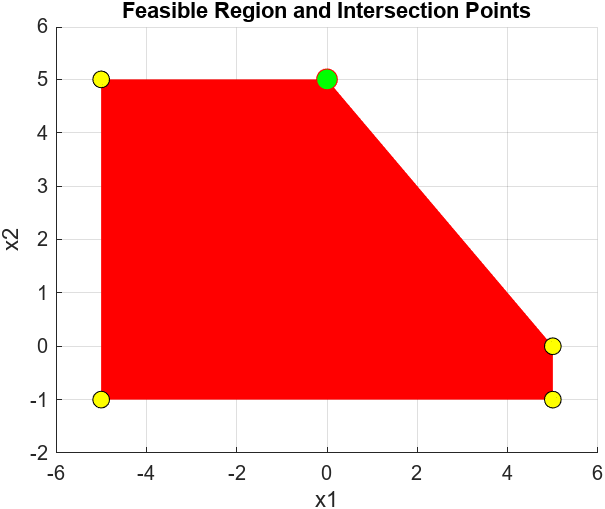
\includegraphics[width=1\linewidth]{../img/Q2_1}
	\caption{}
	\label{fig:q21}
\end{figure}

پاسخ بهینه برای تابع هزینه، با جایگذاری نقاط در آن و انتخاب مقدار کمینه به دست می آید.

\[
(x_1 = 0.00, x_2 = 5) , \quad f(x_1, x_2) = 5
\]

\section{پاسخ سوال 2}

yjtjtyjg
